\documentclass[letterpaper,11pt]{article}
\usepackage[margin=2cm]{geometry}

\usepackage{graphicx}
\usepackage{amsmath}
\usepackage{amsfonts}
\usepackage{amssymb}
\usepackage[colorlinks]{hyperref}

\title{\textbf{Pose Fusion with Chain Pose Graphs for Automated Driving}}
\author{HMW-Alexander}

\begin{document}
	
\maketitle

\tableofcontents
\newpage

\href{./beamer.pdf}{Beamer}

\begin{center}\rule{\textwidth}{1pt}\end{center}
\section{Basic Information}

\subsection{Authors}

\begin{itemize}
	\item \textbf{Christian Merfels} is with Volkswagen Group Research, Wolfsburg, and Institute of Geodesy and Geoinformation, University of Bonn, Germany.
	\item \textbf{Cyrill Stachniss} is with Institute of Geodesy and Geoinformation, University of Bonn, Germany.
\end{itemize}

\subsection{Conference}

2016 IEEE/RSJ International Conference on Intelligent Robots and Systems (IROS)

\subsection{Abstract}

\begin{itemize}
	\item Combining multiple localization systems in a \textbf{plug and play manner}.
	\item Formulate this approach as a \textbf{sliding window pose graph}.
	\item The pose fusion approach scales from a filtering-based to a batch solution by increasing the size of the sliding window.
	\item The experiment runs at 20Hz on both simulated and real data.
\end{itemize}

\subsection{Keywords}

\begin{center}\rule{\textwidth}{1pt}\end{center}
\section{Introduction}

\subsection{Problem \& Solution}

Individual localization system is not enough, and the combination of orthogonal localization systems is more powerful.

\subsection{Objective}

This paper provides an approach to multi-sensor data fusion decouples the localization from the fusion task, which eneables the ability to incorporate third-party localization modules for which source code is unavailable.

\subsection{Formulation}

A coarse localization (red triangles), a precise but only temporary available localization (blue triangles), and odometry as dead reckoning trajectory (blue) are used to estimate the true trajectory (red) of a vehicle. The estimated poses are shown as black triangles: the goal is to approximate the unknown red line as closely as possible with the black triangles.

\begin{figure}[!ht]
	\centering
	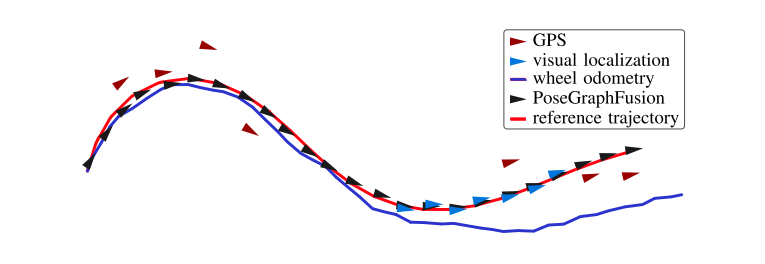
\includegraphics[width=15cm]{./img/posefusion.png}
\end{figure}

\subsection{Contributions}

\begin{itemize}
	\item efficient sensor fusion of generic odometry and global pose inputs $\Rightarrow$ an intuitive architecture for pose estimation and timing issues.
	\item graph construction algorithm $\Rightarrow$ a sparse block-tridiagonal structure of the system matrix $\Rightarrow$ fast solution
\end{itemize}

\begin{center}\rule{\textwidth}{1pt}\end{center}
\section{Related Work}

\subsection{Multi-sensor data fusion for navigation systems}

\begin{itemize}
	\item \textbf{filtering-based approaches}: Kalman filter and its variants
	\begin{itemize}
		\item feature: rely at a very early stage on the Markov assumption and marginalize all older information
		\item problem: prematurely incorporating the linearization error.
	\end{itemize}
	\item \textbf{sliding window smoothing algorithms}: compute the maximum likelihood (ML) estimate by nonlinear least squares optimization to a Bayesian network, Markov random field (MRF), or factor graph.
	\begin{itemize}
		\item feature: consider all past measurements up to the current one; and also consider future measurements for offline batch optimization.
		\item solution: online batch optimization becomes feasible through the usage of incremental smoothing techniques, such as iSAM2\footnote{M. Kaess, H. Johannsson, R. Roberts, V. Ila, J. Leonard, and F. Del- laert, ``iSAM2: Incremental Smoothing and Mapping using the Bayes tree," Int. Journal of Robotics Research, pp. 216–235, 2012.}, that recalculate only the part of the graph that is affected by new measurements.
		\item Some implementations keep the size of the graph bounded by simply discarding older nodes and edges, thus potentially obtaining overconfident estimates.
	\end{itemize}
\end{itemize}

\subsection{Methodical origin}

\begin{itemize}
	\item Sibley et al.\footnote{G. Sibley, L. Matthies, and G. Sukhatme, ``SlidingWindow Filter with Application to Planetary Landing," Journal of Field Robotics, vol. 27, no. 5, pp. 587–608, 2010}, who are the first to introduce the concept of a slibing window filter in the context of robotics.
	\item Differences:
	\begin{itemize}
		\item apply this to the use case of pose fusion
		\item special design for a faster way of solving the nonlinear least squares equations, performing marginalization, and estimating the uncertainty of the output.
		\item provide a way of semantically reasoning about the prior information arising from marginalization by deriving a prior node.
	\end{itemize}
\end{itemize}

\begin{center}\rule{\textwidth}{1pt}\end{center}
\section{Pose Graph Fusion}

\subsection{Nonlinear least squares problem}

This paper exploits the state-of-the-art graph optimization framework g2o\footnote{R. K¨ ummerle, G. Grisetti, H. Strasdat, K. Konolige, and W. Burgard, ``g2o: A General Framework for Graph Optimization," in Proc. IEEE Int. Conf. Robotics and Automation (ICRA), 2011, pp. 3607–3613.}.

The key idea is that given the state vector $x=(x_1^T, ..., x_m^T)^T$ and a set of measurements, where $z_{ij}$ is the mean and $\Omega_{ij}$ is the information matrix\footnote{\url{https://en.wikipedia.org/wiki/Fisher_information}} of a single measurement relating $x_i$ to $x_j$, least squares estimation seeks the state
\begin{equation}
x^*=\arg\min_x{\sum_{i,j}e_{ij}^T\Omega_{ij}e_{ij}}
\label{eq:state}
\end{equation}
that best explains all measurements given the $\mathit{l}_2$ norm. The vector error function $e_{ij}=e(x_i,x_j,z_{ij})$ measures how well the constraint from the measurement $z_{ij}$ is satisfied. Solving $(\ref{eq:state})$ requires iteratively solving a linear system with the system matrix\footnote{\url{https://en.wikipedia.org/wiki/State-space_representation}} $H$ and the right-hand side vector $b$ such that
$$H=\sum_{i,j}{J_{ij}(x)^T\Omega_{ij}J_{ij}(x)}$$
$$b^T=\sum_{i,j}e_{ij}^T\Omega_{ij}J_{ij}(x)$$
where $J_{ij}(x)$ refers to the Jacobian\footnote{\url{https://en.wikipedia.org/wiki/Jacobian_matrix_and_determinant}} of the error function computed in state $x$.

\subsection{Sliding window chain pose graph fusion}

\subsubsection{About the online state estimation system}

\begin{itemize}
	\item general nonlinear least squares estimation taks into account all available information within the full pose graph
	\item to keep the problem computationally tractable, it is necessary to limit the considered information.
	\item this approach achieves this by marginalizing out prior state state variables and the state vector $x$ in a sliding window pose graph is reduced to the M most recent states $x=(x_{t-M+1}^T,...,x_t^T)^T$.
\end{itemize}

\subsubsection{About the graph structure}

\begin{itemize}
	\item global pose source: measure poses within a global coordinate system, e.g. Universal Transverse Mercator (UTM) coordinate
	\item local pose source:  measure spatial transformations relative to the previous pose, e.g. odometry
	\item hidden nodes (from MRFs): state variables
	\item observed nodes (from MRFs): global pose constraints, connected to hidden nodes to constrain them in the global coordinate frame.
	\item edge between hidden nodes: local pose constraints.
	\item The resulting form or the graph is called \textbf{chain pose graph}.
\end{itemize}

\begin{figure}[!ht]
	\centering
	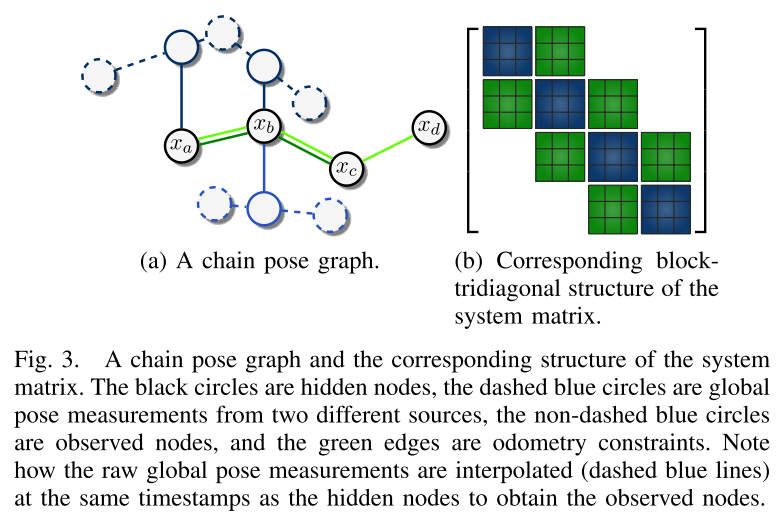
\includegraphics[width=15cm]{./img/posegraph.png}
\end{figure}

\subsubsection{About the algorithm working frequency}

\begin{itemize}
	\item Related graph-based approaches.
	\begin{itemize}
		\item generate a hidden node (state variables) every time a measurement arrives
		\item or tie their generation to a specific pose source
	\end{itemize}
	\item This approach constructs a hidden node every time stamp.
	\begin{itemize}
		\item it queries all global pose sources for measurements and interpolate one observed node per source at the timestamp of the hidden node if measurements are available.
		\item it queries each local pose source to interpolate the edges between all two successive hidden nodes.
		\item enforce a certain matrix structure for H, to include all measurement sources in a generic way independetly of their specific output frequencies, and to a priori relate the number of state variables to the length of the interval of the sliding window.
	\end{itemize}
\end{itemize}

\subsubsection{About the system matrix $H$}

\begin{itemize}
	\item The block-tridiagonal structure is a consequence of the linear temporal ordering of the state variables combined with the fact that edges are at most constructed between successive nodes.
	\item This structure does not produce fill-in in system matrix $H$ after marginalization of the oldest state variables.
	\item Beyond that, even the Cholesky factorization\footnote{\url{https://en.wikipedia.org/wiki/Cholesky_decomposition}} $H=R^TR$, which this paper perform to solve the linear system, does not suffer from fill-in in its triangular matrix $R$ (becomes a band matrix).
	\item The computational complexity of this approach is efficiently solvable in $\mathcal{O}(n)$.
\end{itemize}

\subsection{Time behavior}

\begin{itemize}
	\item Define time behavior as the latency, frequency, and availability of estimate. The output of the PoseGraphFusion is time-triggered.
	\item Difficulties:
	\begin{itemize}
		\item multi-rate sources,
		\item nonconstant input frequencies,
		\item out-of-sequence estimates,
		\item time-varying latencies.
	\end{itemize}
	\item Steps:
	\begin{enumerate}
		\item buffering all incoming data.
		\item preprocessing it before the next graph construction phase.
		\item constructing and optimizing the graph.
		\begin{itemize}
			\item computation time
			\item the most recent state is estimated with a sliding window pose graph over the current set of measurements.
		\end{itemize}
		\item The estimation result is subsequently propagated into the future to the start of the next cycle with a constant turn rate and velocity model.
	\end{enumerate}
	\begin{figure}[!ht]
		\centering
		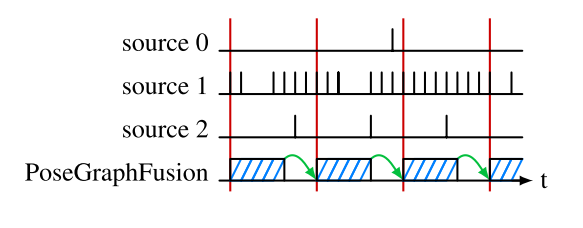
\includegraphics[width=10cm]{./img/timebehavior.png}
	\end{figure}
	\item The backward-forward computations problem of conventional Kalman filtering approaches: to integrate a new measurement, it has to propagate its state back in time to the time of the measurement, apply the measurement, and re-apply all other stored measurements.
\end{itemize}

\subsection{Marginalization in the form of a prior node}

\begin{itemize}
	\item Motivation: limit the amount of hidden nodes to maintain constant runtime complexity.
	\item Problem: Simply removing edges and nodes leads to information loss and is equivalent to conditioning, which potentially leads to overconfidence.
	\item Solution: only marginalize the oldest nodes. This truncates the graph but retains the same information (given te linearization point).
	\item Common method: Computing the Schur complement\footnote{\url{https://en.wikipedia.org/wiki/Schur_complement}} on the system matrix $H$.
	\begin{itemize}
		\item Potential problem: may introduce conditional dependencies between state variables that are connected.
		\item however, the structure of the chain pose graph is able to retain the same sparsity pattern and do not suffer from a denser system matrix after marginalization.
	\end{itemize}
	\item Prior node: this paper says, by exploiting the particular block-tridiagonal matrix structure, it derives the concept of a prior node, which carries the same information as introduced by the Schur complement. Therefore, it is advantageous to construct a prior node for marginalization instead of performing the Schur complement:
	\begin{itemize}
		\item user has the possibility to understand how the prior information affects the rest of the graph.
		\item it allows to store and load the optimization problem with solely the help of its graph representation.
		\item it opens up the possibility to explicitly apply a robust kernel on the cost function of the prior node and to adjust the uncertainty of the prior information based on context.
	\end{itemize}
\end{itemize}

\subsubsection{Effect of the Schur complement on chain pose graphs}



\subsubsection{Derivation of the prior node}
***
Still working on the mathematical details... (planned 11/11)
***

\subsection{Assessing the uncertainty of the fused estimate}

The optimization assigns to the hidden nodes the global poses which best satisfy all constraints. Solving the nonlinear least squares problem of the pose fusion with a sparse solver typically involves computing the Cholesky factorization $H=R^TR$, where $R$ is an upper triangular matrix with entries $r_ij$. Following the referred paper [13]\footnote{M. Kaess and F. Dellaert, ``Covariance Recovery from a Square Root Information Matrix for Data Association," Robotics and Autonomous Systems, pp. 1198–1210, 2009.}, the uncertainty matrix of the hidden nodes $H^{-1}$ with entries $H_{ij}^{-1}$ is obtained by the recursive formula:
\begin{equation}
\begin{array}{rcl}
H_{ii}^{-1} & = & \frac{1}{r_{ii}}\left[\frac{1}{r_{ii}}-\sum_{\begin{array}{c}
	k=i+1 \\
	r_{ik} \neq 0 \\
	\end{array}}^{n}{r_{ik}H_{ki}^{-1}}\right] \\
H_{ij}^{-1} & = & \frac{1}{r_{ii}}\left[-\sum_{\begin{array}{c}
	k=i+1 \\
	r_{ik} \neq 0 \\
	\end{array}}^{j}{r_{ik}H_{kj}^{-1}}-\sum_{\begin{array}{c}
	k=j+1 \\
	r_{ik} \neq 0 \\
	\end{array}}^{n}{r_{ik}H_{jk}^{-1}}\right]
\end{array}
\end{equation}
The formula yields an $\mathbb{O}(n)$ time complexity with $n$ being the number of state variables. It becomes constant time for sliding window pose graphs as the number of state variables is upper bounded by a constant value.

\subsection{Noise correlations between input sources}

\begin{itemize}
	\item This method needs to apply appropriate preprocessing (covariance intersection\footnote{S. J. Julier and J. K. Uhlmann, ``A non-divergent estimation algorithm in the presence of unknown correlations," in Proc. Amer. Control Conf. (ACC), 1997, pp. 2369–2373.}) if noise is correlated between input sources:
	\begin{itemize}
		\item different input source build up on the same sensor data
		\item the same algorithm runs on two physically different sensors.
	\end{itemize}
	\item Combine groups of sources with correlated noise into a single consistent estimate.
\end{itemize}

\section{Evaluation}

Baseline: the online ML (maximum likelihood) estimate, scaling from a filtering to a batch least squares solution.

\subsection{Experiment on a real prototype vehicle}

\subsubsection{Settings}
\begin{itemize}
	\item global sources:
	\begin{itemize}
		\item source 0: coarse LiDAR scans to a globally referenced point cloud. (3rd-party)
		\item source 1: GPS (3rd-party)
		\item source 2: visual localization system with a globally referenced feature map.
	\end{itemize}
	\item local source: wheel odometry.
	\item sliding window size: $M=1000$
	\item temporal resolution: $\Delta t=25ms$
	\item experiment route: $16km$ in rural and urban areas in Germany.
\end{itemize}

\subsubsection{Pose estimate quality}
Baseline: batch solution.\\
Noises are not independently distributed with zero mean and the uncertainty models are unknown. 
\begin{itemize}
	\item source 0: $RMS=1.06m$
	\item source 1: $RMS=1.23m$
	\item source 2: $RMS=0.28m$
	\item PoseGraphFusion: $RMS=0.38m$
\end{itemize}
\begin{figure}[!ht]
	\centering
	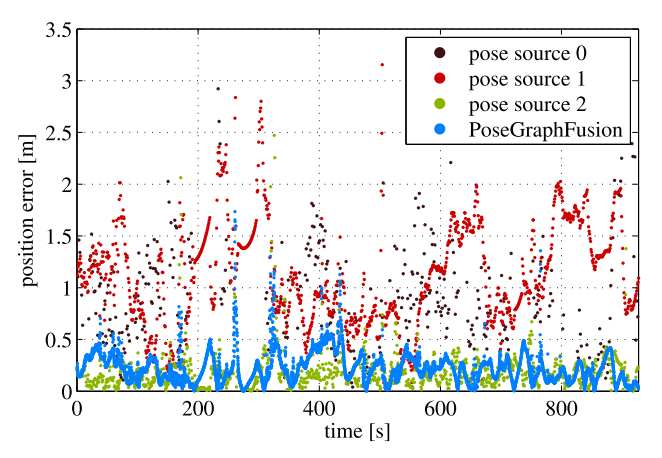
\includegraphics[width=10cm]{./img/error.png}
\end{figure}

\subsubsection{Latency and availability}
Latency: $\leq 10ms$.\\
Availability:
\begin{itemize}
	\item source 0: $66.98\%$
	\item source 1 with odometry: $100\%$
	\item source 2: $97.76\%$
	\item PoseGraphFusion: $100\%$
\end{itemize}

\subsubsection{Runtime performance}
a single core of a laptop with an Intel i7-4800QM processor
\begin{figure}[!ht]
	\centering
	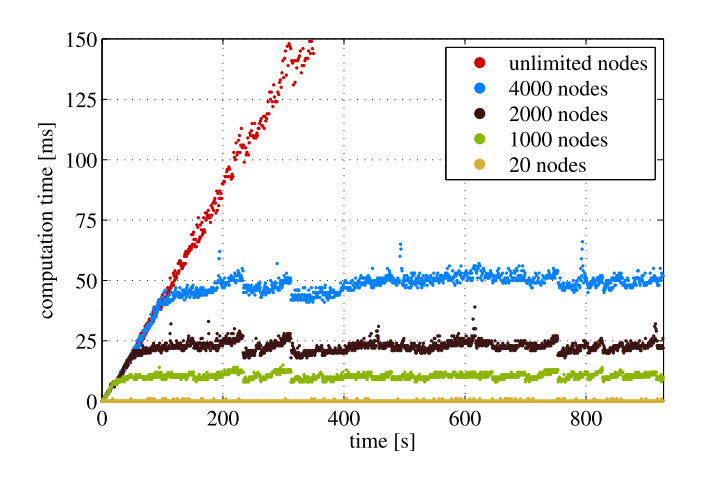
\includegraphics[width=8.5cm]{./img/runtime.png}
	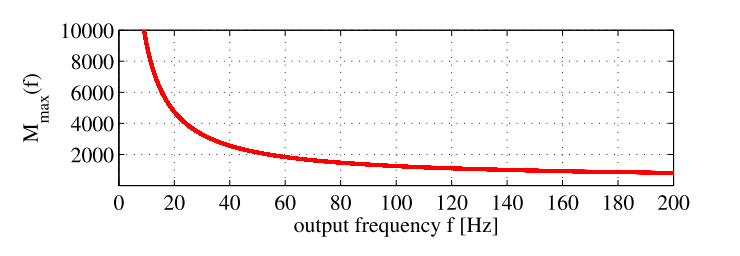
\includegraphics[width=8.5cm]{./img/relationship.png}
\end{figure}

\subsection{Simulated input data}

\subsubsection{Number of hidden nodes v.s. accuracy}
Larger sliding window size $\Rightarrow$ more accurate result
\begin{figure}[!ht]
	\centering
	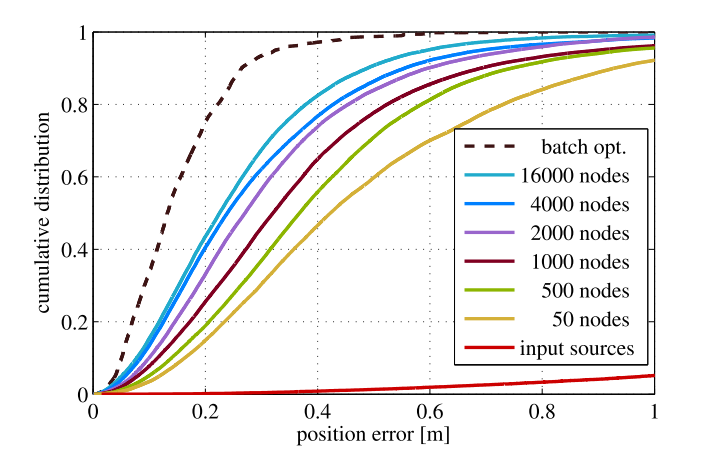
\includegraphics[width=10cm]{./img/accuracy.png}
\end{figure}

\subsubsection{Number of pose sources v.s. accuracy}
More pose sources $\Rightarrow$ more accurate result
\begin{figure}[!ht]
	\centering
	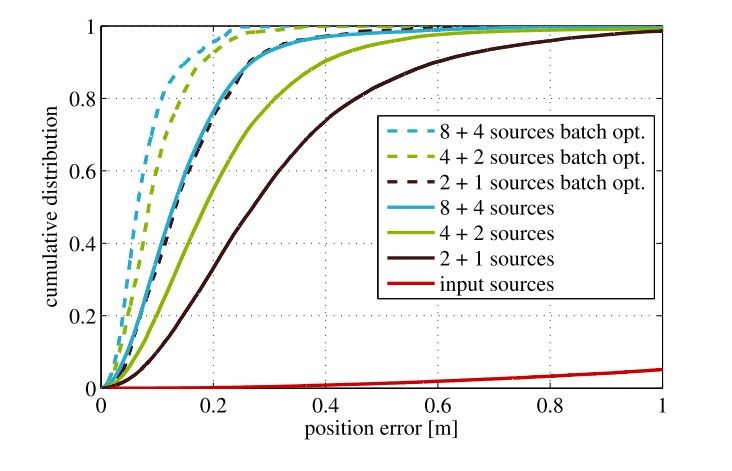
\includegraphics[width=10cm]{./img/sources.png}
\end{figure}

\section{Conclusion}
\begin{itemize}
	\item Motivation: the need for fast, recent, accurate, and highly available pose estimates.
	\item Method: a sliding window graph-based optimization scheme.
	\item The design of chain pose graphs for efficient optimization.
\end{itemize}

\end{document}